The European Organisation for Nuclear Research (CERN\footnote{The name CERN is derived from the acronym for the French Conseil Europ\'{e}en pour la Recherch Nucl\'{e}aire.}) was founded in 1954 and is based in the suburb of Geneva on the Franco\textendash Swiss border.
The main function of CERN is to provide particle accelerators and detectors for high-energy physics research.
The physicists and engineers at CERN are probing the fundamental structure of the universe using the world's largest and most complex scientific facility \textemdash \ the \textit{Large Hadron Collider} (LHC)~\cite{Evans:2008zzb}.
In the LHC, the particles are boosted to high energies and collide at close to the speed of light.
The results of the collisions are recorded by the various detectors.
There are seven experiments at the LHC.
The biggest of these experiments are \textit{ATLAS} (A Toroidal LHC ApparatuS)~\cite{Aad:2008zzm} and \textit{CMS} (Compact Muon Solenoid)~\cite{Chatrchyan:2008aa} which use general-purpose detectors to investigate a broad physics programme ranging from the search for the Higgs boson to extra dimensions and particles that could make up dark matter.
The \textit{ALICE} (A Large Ion Collider Experiment)~\cite{Aamodt:2008zz} experiment is designed to study the physics of quark-gluon plasma form and the \textit{LHCb} (Large Hadron Collider beauty)~\cite{Alves:2008zz} experiment specialises in investigating of CP violation\footnote{The CP violation is violation of the charge conjugate and parity symmetry which says if a particle is interchanged with its anti-particle and its spatial coordinates are inverted, then the physics laws should be the same.} by studying the $b$-quark.
These four detectors sit underground in huge caverns of the LHC ring.
The rest three experiments, \textit{TOTEM}~\cite{Anelli:2008zza}, \textit{LHCf}~\cite{Adriani:2008zz}, and \textit{MoEDAL}~\cite{Pinfold:2009oia}, are smaller.
The TOTEM (TOTal Elastic and diffractive cross section Measurement)~\cite{Anelli:2008zza} experiment aims at the measurement of total cross section, elastic scattering, and diffractive dissociation.
The LHCf (Large Hadron Collider forward)~\cite{Adriani:2008zz} experiment is intended to measure the neutral particle produced by the collider using the forward particles.
The prime motivation of the MoEDAL (Monopole and Exotics Detector at the LHC)~\cite{Pinfold:2009oia} experiment is to search directly for the magnetic monopole.
An overview of the LHC is described in Section~\ref{sec:ae_LHC} and the detector apparatus of the ATLAS experiment is outlined in Section~\ref{sec:ae_ATLAS}.

%%%
%%%
%%%

\section{The Large Hadron Collide}
\label{sec:ae_LHC}
The LHC~\cite{Evans:2008zzb} is the world's largest and most powerful accelerator which accelerates and collides protons in a 26.7~km circumference crossing the Franco\textendash Swiss border 100~m underground.
Built in the tunnel of the former \textit{LEP} (Large Electron\textendash Positron), the LHC is capable of colliding protons as well as heavy ions.
Comparing with the LEP which collides electrons and positrons, the advantage of the LHC is the lower energy loss\footnote{The energy loss for protons is about eleven orders of magnitude smaller than the electrons.} in the synchrotron radiation, such that higher energies can be reached by the LHC.
The LHC is designed for collisions at a centre-of-mass energy $\sqrt{s}=14$~{\TeV} and an instantaneous luminosity of $\mathcal{L} =10^{34}~\textrm{cm}^{-2}\textrm{s}^{-1}$.
Figure~\ref{fig:ae_CERN_accelerator_complex} shows the infrastructure of the LHC and the pre-accelerator system.

\begin{figure}[htbp]
    \begin{center}
        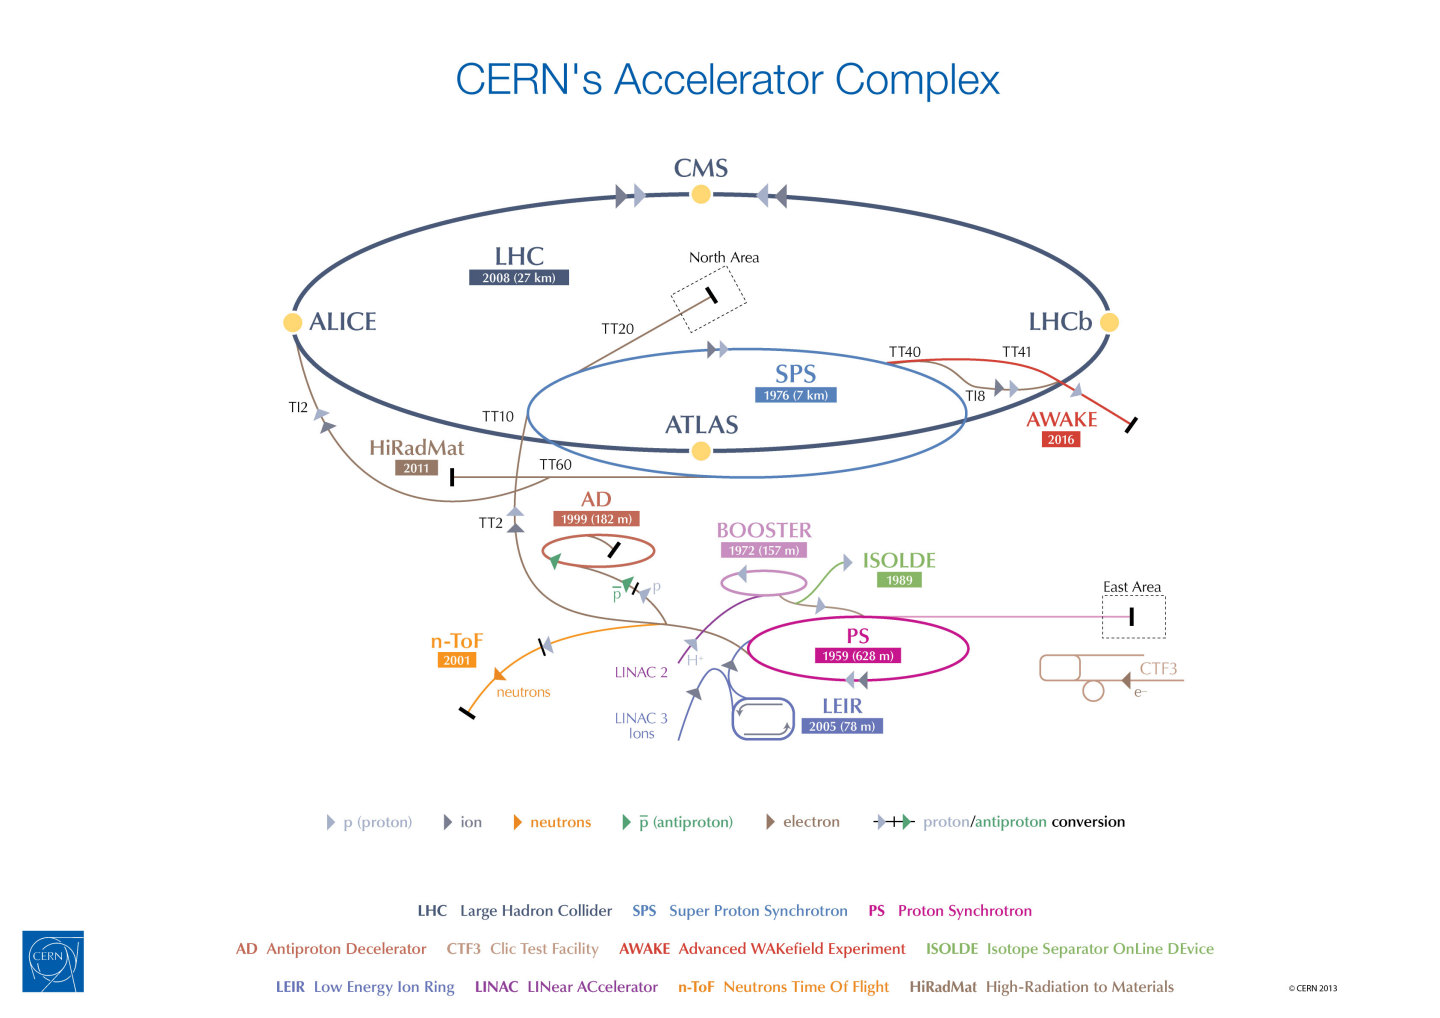
\includegraphics[scale=0.4]{CERN's-accelerator-complex2013.jpg}
        \caption{The accelerator complex at CERN~\cite{Marcastel:1621583}.}
        \label{fig:ae_CERN_accelerator_complex}
    \end{center}
\end{figure}

The protons are extracted by ionisation from a hydrogen source and are accelerated to 50~{\MeV} by the linear accelerator \textit{LINAC2}.
Then they are injected into the \textit{Proton Synchrotron Booster} (PSB) where the proton energies are increased to 1.4~{\GeV} before they enter the \textit{Proton Synchrotron} (PS) which accelerates the protons to 25~{\GeV}.
Next, the proton energies are increasing to 450~{\GeV} in the \textit{Super Proton Synchrotron} (SPS). 
Finally, the protons are split into two beams and enter the LHC where the two beams run in two adjacent beam pipes with opposite directions.
In order to keep the protons on the circular trajectory in the LHC, 1232 superconducting dipole magnets~\cite{Rossi:2003np} generate a magnetic field strength of 8.33~T to bend the proton beams in eight arcs.
Additionally, 392 quadrupole magnets~\cite{Rossi:2003np} are installed to focus the beam.
A cryogenic system running with super-fluid helium-4 is used to cool down the superconducting magnets to a temperature of 1.7~K.

For a given physics process, the event rate is proportional to the cross section $\sigma$ of this process
%
\begin{equation}
    \frac{dN}{dt} = \mathcal{L}\cdot\sigma
\end{equation}
%
where $N$ is the number of events and $\mathcal{L}$ denotes the luminosity of the beam.
The luminosity of the beam, $\mathcal{L}$, can be calculated by
%
\begin{equation}
    \mathcal{L} = \frac{N^{2} f}{4 \pi \sigma_{x} \sigma_{y}} \cdot F
\end{equation}
%
where $N$ is the number of protons, $f$ is the bunches crossing frequency, and the $\sigma_{x}$ and $\sigma_{y}$ are the $x$ and $y$ components for cross section $\sigma$.
The geometric luminosity reduction factor, $F$, is related to the crossing angle at the \textit{interaction point} (IP).
Considering a beam consisting of $1.15 \times 10^{11}$ protons with bunching spacing of 25~ns, the transversal size of the bunch at IP $16\times 10^{-4}$~cm, and taking the geometric luminosity reduction factor as 1, the design luminosity of $10^{34}$~cm$^{-2}$s$^{-1}$ can be reached.

The first beam was circulated through the collider on the morning of 10 September 2008~\cite{CERN-COURIER-Sep192008}.
However, a magnet quench incident occurred on 19 September 2008 and caused extensive damage to over 50 superconducting magnets, their mountings, and the vacuum pipe.
Most of 2009 was spent on repairs the damage caused by the magnet quench incident and the operations resumed on 20 November of that year.
The first phase of data-taking (Run 1) started at the end of 2009 and the beam energy was increased to a centre-of-mass $\sqrt{s}=7$~{\TeV} in 2011 and $\sqrt{s} = 8$~{\TeV} in 2012.
The total integrated luminosity of 5.46~{\ifb} was collected in 2011 and of 22.8~{\ifb} was collected in 2012.
Since 13 February 2013 the LHC was in the Long Shutdown 1 (LS1) phase for maintenance and upgrades.
On 5 April 2015, the LHC restarted and was operating at a centre-of-mass energy $\sqrt{s}=13$~{\TeV} throughout the Run 2 phase\footnote{The Run 2 data-taking started from 2015.}.

%%%
%%%
%%%

\section{The ATLAS experiment}
\label{sec:ae_ATLAS}
The ATLAS\footnote{A Toroidal LHC Apparatus} detector~\cite{Aad:2008zzm} is a multi-purpose detector housed in its cavern at point 1 at the LHC~\cite{Evans:2008zzb}.
It is the largest experiment at the LHC with a length of 44~m, a diameter of 25~m, and a weight of approximately 7000 tonnes.
It consists of three high precision sub-detector systems which are arranged concentrically around the interaction point and in forward and backward symmetrically.
Related to this symmetry, the ATLAS detector is sectioned into the central barrel region with one end-cap region perpendicular to the beam pipe on either side.
Figure~\ref{fig:ae_ATLAS_detector} shows an overview of the ATLAS detector with its major components.

\begin{figure}[htbp]
    \begin{center}
        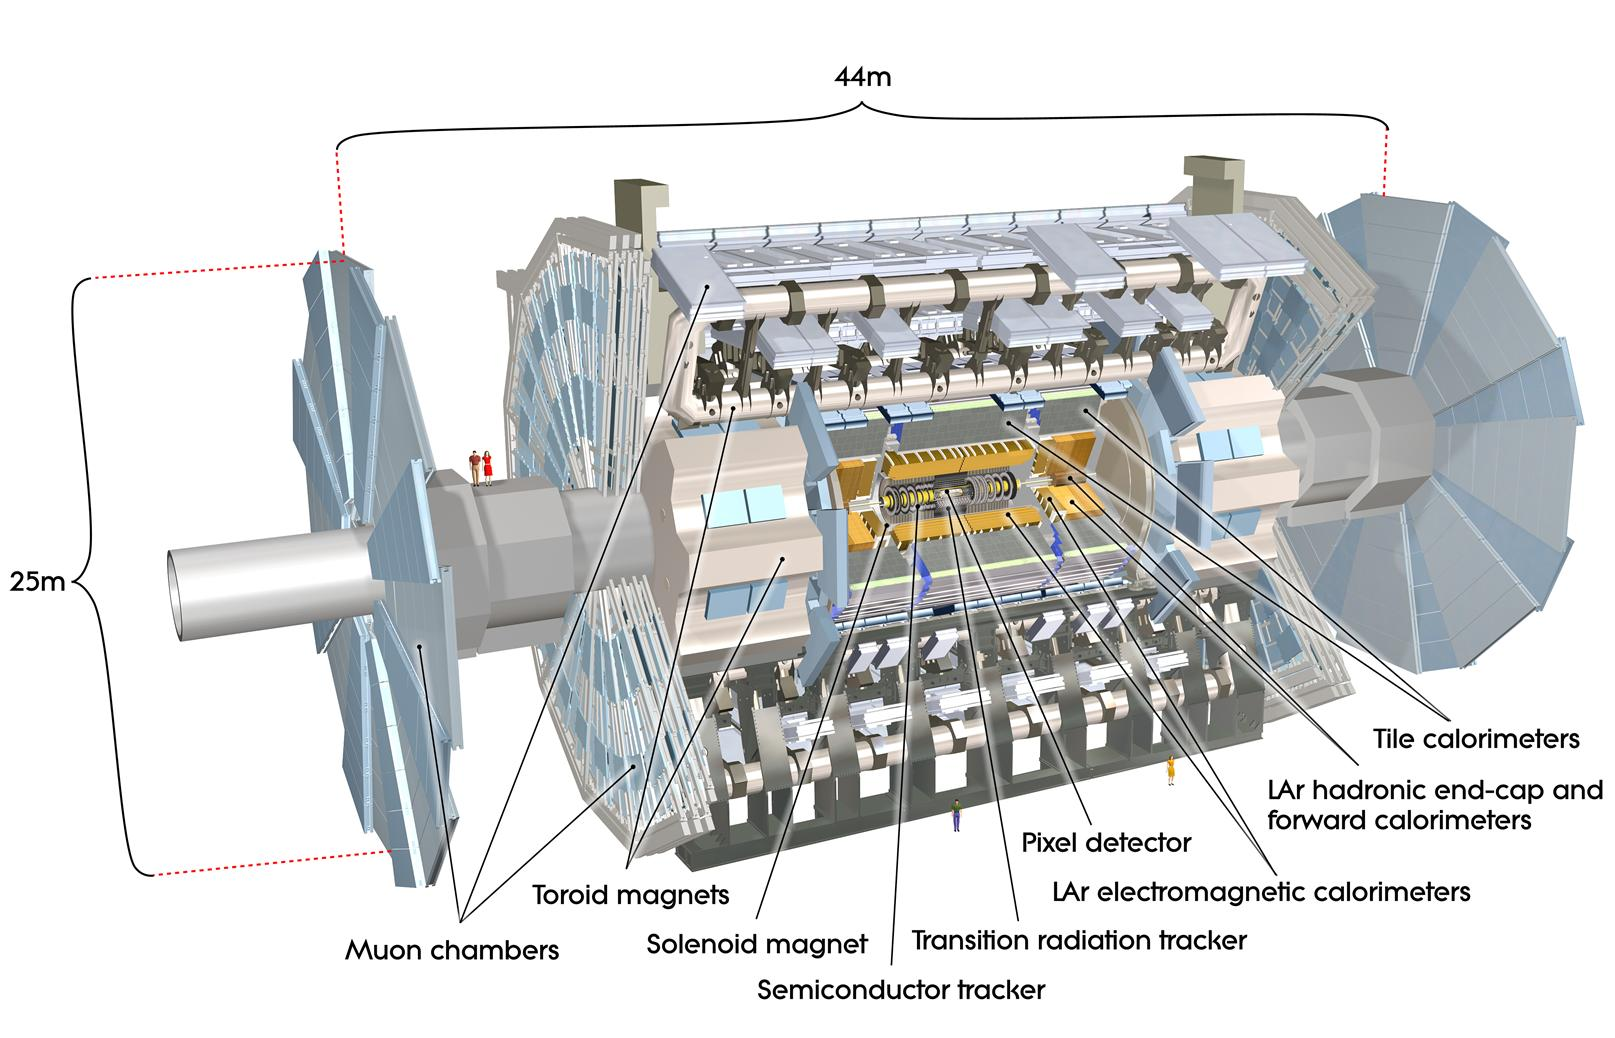
\includegraphics[scale=0.4]{0803012_01-A4-at-144-dpi.jpg}
        \caption{Overview of the ATLAS detector~\cite{Aad:2008zzm}.}
        \label{fig:ae_ATLAS_detector}
    \end{center}
\end{figure}

The ATLAS detector is designed to record the proton-proton interactions delivered by the LHC.
It can identify particles and measure their tracks and energies with very high precision, therefore, it is sensitive to large areas of particle physics phenomena from the precision measurement of the  Standard Model to beyond the Standard Model (BSM).
The detector is constituted by three sub-detector systems and the magnet system.
The innermost part of the detector is called the \textit{inner detector} which identifies and reconstructs the charged particles as well as the primary and secondary vertices.
Around it, the \textit{calorimeter} system is built as a cylindrical barrel with caps at each end to measure the particle energies.
The detector is completed by the \textit{muon spectrometer} which performs identification and measurement of momenta of muons.
The magnetic system produces a field of $B$ = 0.5~T and $B$ = 1~T at barrel and two end-cap, respectively.
The detector has to withstand large collision rates with approximately 1000 particles per collision, therefore, a fast readout and a three-level trigger system are implemented to reduce the event rate from 40~MHz to 200~Hz.
The ATLAS coordinate system and the detail of each sub-detector systems are described in the following sections.

%%%
%%%
%%%

\subsection{The ATLAS coordinate system}
\label{subsec:ae_atlas_coordinate}
ATLAS uses a \textit{right-handed coordinate system} with its origin at the nominal proton-proton interaction point (IP) in the centre of the detector and the $z$-axis along the beam pipe.
Along the $z$-axis the detector is divided into side-A (positive $z$) and side-C (negative $z$).
The positive $x$-axis is defined by the direction pointing from the interaction point to the centre of the LHC ring, and the positive $y$-axis points upward.%Cylindrical coordinates $(r, \phi)$ are used in the transverse plane.
The azimuthal angle $\phi$ is measured around the beam pipe  and the polar angle $\theta$ is the angle from the $z$-axis.
The transverse momentum $p_{\mathrm{T}}$, the transverse energy $E_{\mathrm{T}}$ and the missing transverse
energy $E_{\mathrm{T}}^{\mathrm{miss}}$ are defined in the transverse plane\footnote{$x-y$ plane}, here exemplary for $p_{\mathrm{T}}$
%
\begin{equation}
    p_{\mathrm{T}}= \sqrt{p_{x}^{2} + p_{y}^{2}}
\end{equation}
%
An important quantity in hadron collider physics is the \textit{rapidity}, $y$, because of the invariance $y$ under Lorentz boosts in the longitudinal direction.
The rapidity is defined as
%
\begin{equation}
    y = \frac{1}{2} \ln\Big[\frac{E + p_{z}}{E - p_{z}}\Big]
\end{equation}
%
where $E$ denotes the particle energy and $p_{z}$  is the component of the momentum along the beam direction.
Since mainly leptons can be considered massless in respect to the nominal centre-of-mass energy, the pseudorapidity, $\eta$, is used in stead of using the $y$.
For a massless particle, the \textit{pseudorapidity}, $\eta$, depends on the polar angle $\theta$ through
%
\begin{equation}
    \eta = - \ln \tan \frac{\theta}{2}
\end{equation}
%
For a particle with the energy $E$ much larger than its mass, the approximation $E \approx |\vec{p}|$ is valid.
The distance, $\Delta R$, between two objects in the $\eta-\phi$ plan is given by
%
\begin{equation}
    \Delta R = \sqrt{\Delta \eta^{2} + \Delta \phi^{2}}
\end{equation}
%
where $\Delta \eta$ and $\Delta \phi$ are the difference in pseudorapidity and azimuthal angle, respectively.

%%%
%%%
%%%

\subsection{The inner detector and tracking system}
\label{subsec:ae_inner_detector}
The \textit{inner detector} (ID) consists of three sub-detectors: the \textit{pixel} detector, the \textit{semi conductor tracker}  (SCT), and the \textit{transition radiation tracker} (TRT).
The main purpose of the inner detector is to provide high precision measurements of the tracks of particles and to reconstruct the primary and secondary vertices.
Each sub-detectors are composed of several layers of material which interacts with the charged particles when the charged particles penetrate the layers.
A  2~T magnetic field generated by the central solenoid parallel to the beam axis is applied to bend the charged particles using the Lorentz force.
By using the radius $r$ of the curvature of the tracks, the magnetic field strength $B$, and the charge of the particle $q$, we can calculate the magnitude of the transverse momentum \pt
%
\begin{equation}
    \pt = |q|Br
\end{equation}
%
The layout of the inner detector is illustrated in Figure~\ref{fig:ae_inner_detector} and the detail of sub-detectors are described in the following paragraphs.

\begin{figure}[htbp]
    \begin{center}
        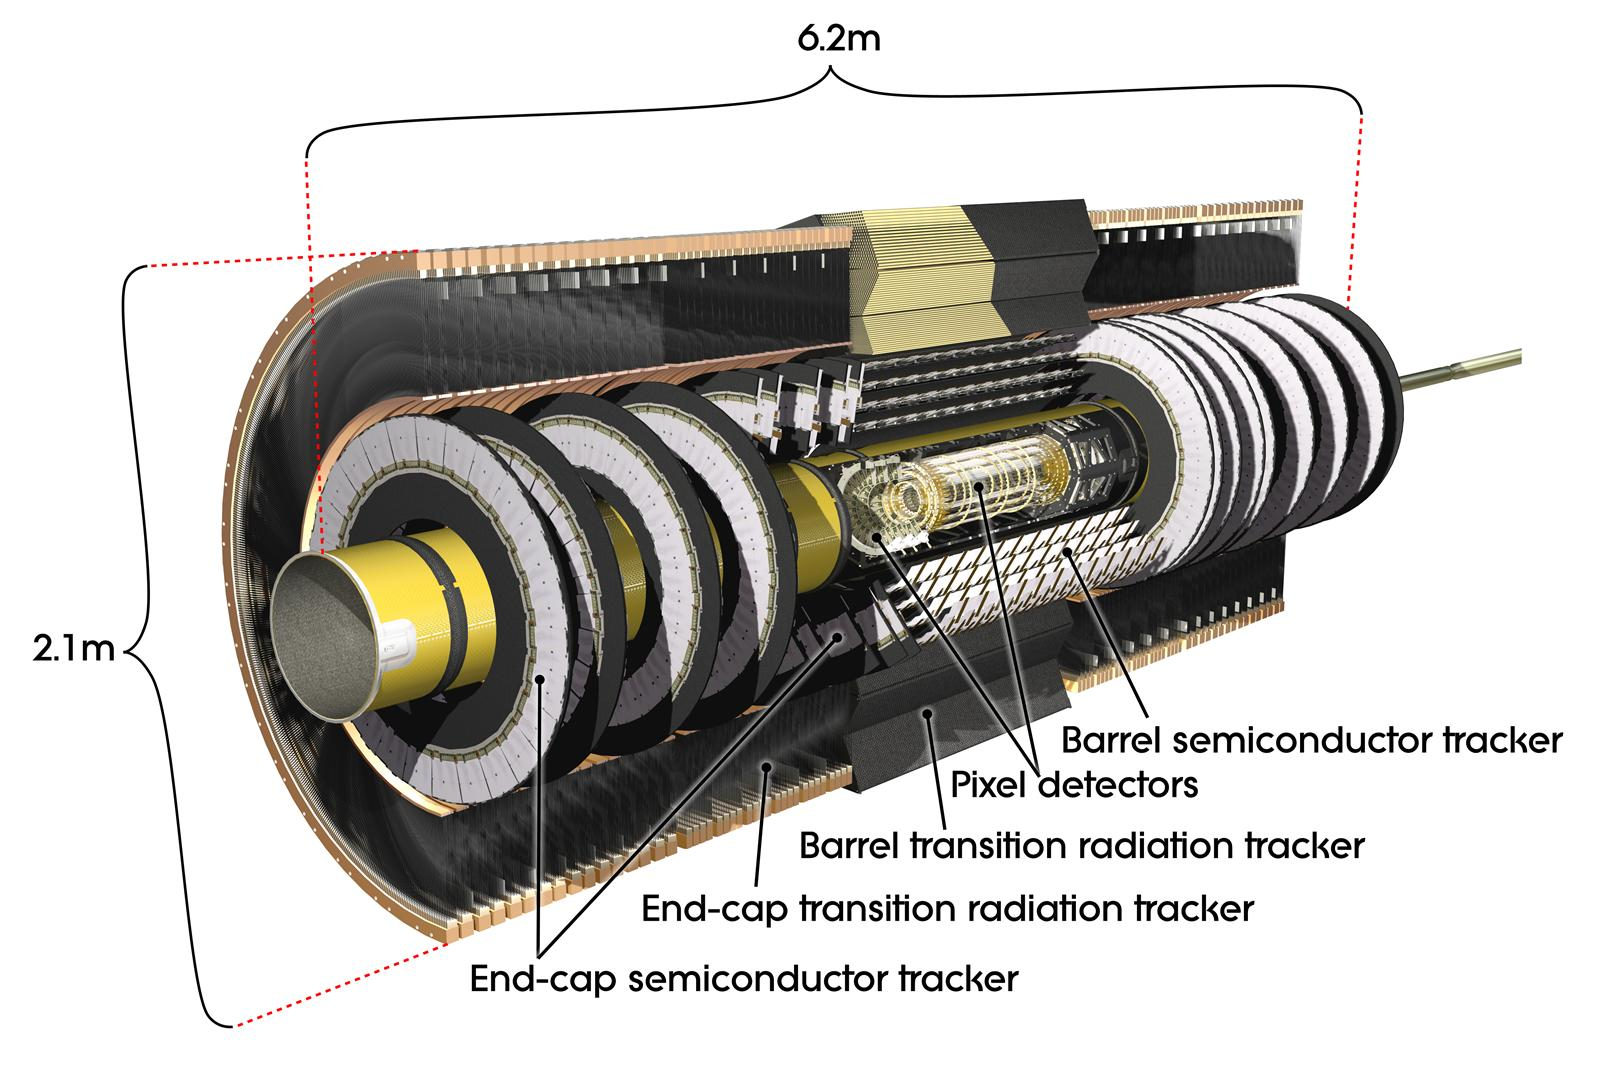
\includegraphics[scale=0.4]{0803014_01-A4-at-144-dpi.jpg}
        \caption{Cut-away view of the ATLAS inner detector~\cite{Aad:2008zzm}.}
        \label{fig:ae_inner_detector}
    \end{center}
\end{figure}

%%%
%%%
%%%

\subsubsection{Pixel detector}
\label{subsubsec:ae_pixel}
The innermost part of the entire ATLAS detector components is the \textit{pixel} detector which is composed of three barrel layers and three end-cap disks on each side.
The three cylindrical barrel layers around the beam axis have radial positions of 50.5~mm, 88.5~mm, and 122.5~mm respectively and they are made of 22, 38, and 52 identical staves respectively.
Each stave is inclined with azimuthal angle of 20 degrees and is composed of 13 pixel modules with 46,080 readout channel per module.
The size of each pixel is $50 \times 400~\mu m^{2}$ in $R-\phi \times z$.
In the forward region, three disks on each side equip the modules identical to the barrel modules, except the connecting cables. 
The total 1,744 modules in the pixel detector lead to nearly 80 million channel readout and provide the intrinsic accuracy of $10~\mu m$ in $R-\phi$ plane and $115~\mu m$ in $z$ direction covering the region $|\eta| < 2.5$. 

%%%
%%%
%%%

\subsubsection{Semi conductor tracker}
\label{subsubsec:ae_sct}
On the top of the pixel detector is the \textit{semi conductor tracker} (SCT) which is a silicon strip detector.
There are about 6.3 million readout channels which are arranged in 4088 microstrips.
The intrinsic accuracies per sensor is $17~\mu m$ in $R-\phi$ and $580~\mu m$ in $z$ direction for the barrel and in $R$ for the  disks, respectively.
Similar to the pixel detector, the SCT covers the region $|\eta| < 2.5$ and consists of 8 strip layers in barrel and a total of 9 discs in the end-cap region on each side.
No track reconstruction is possible beyond the covered pseudorapidity range.
Therefore, the electrons cannot be distinguished from photons above $|\eta| > 2.5$ region.

%%%
%%%
%%%

\subsubsection{Transition radiation tracker}
\label{subsubsec:ae_trt}
The outermost component of the inner detector is the \textit{transition radiation tracker} (TRT) which consists of 4~mm diameter straw tubes filled with the xenon-based gas mixture.
The gas mixture are ionised by charged particles when they penetrates the straws.
The ionised electrons drift to the cathode because a high voltage is applied on the tungsten wire in the center of the straw tube.
Therefore, the TRT allows the enhanced electron identification, momentum measurement, vertex measurement.
In the barrel region, the straws are surrounded by polypropylene fibres and are divided into two halves at $|\eta|=0$.
In the end-caps, the straws are arranged radially and surrounded by foils as a transition radiation element.
They are read out at two sides and at the center of the TRT with the total number of the readout channels of TRT are approximately 350,000.
The TRT only provides information in the $R-\phi$ plane with an intrinsic accuracy of 130~$\mu$m per straw and covers a range up to $|\eta| < 2.0$. 

%%%
%%%
%%%

\subsubsection{Solenoid magnet}
\label{subsubsec:ae_magnetic}
A superconducting solenoid magnet encloses the inner detector and produces a 2~T magnetic field to bend the trajectories of the charged particles.
A cooling system is used and shared with the \textit{electromagnetic calorimeter} (Section~\ref{subsec:ae_calorimeter}) to reduced the deterioration of the energy measurement.

%%%
%%%
%%%

\subsection{The calorimeters}
\label{subsec:ae_calorimeter}
The calorimeters are used to measure the energy of particles, such as electrons, photons, and jets.
Besides muons and neutrinos, all other particles interacting electromagnetically or hadronically are stopped in the calorimeters by absorbing their energy.
Not only charged particles but also neutral particles such as photons and neutral hadrons can be detected in the calorimeters.
By requiring highly hermiticity of the calorimeters, the missing energy \met can be reconstructed precisely as negative vectorial sum of all energy deposits.
The ATLAS calorimeter system is placed between the inner detector (Section~\ref{subsec:ae_inner_detector}) and the muon spectrometer (Section~\ref{subsec:ae_the_muon_spectrometer}).
The ATLAS calorimeter system consists of an inner \textit{electromagnetic calorimeter} and an outer \textit{hadronic calorimeter} together with the \textit{forward calorimeter}.
The electromagnetic calorimeter and hadronic calorimeter are \textit{sampling calorimeters} which consist of two different materials alternately.
An absorber material is used to enhance the particle showers\footnote{The shower is the cascade of secondary particles produced by the high-energy particle interacting with dense material.} and a highly ionisable active medium is used to measure the deposited energy.
Because only the energies deposited in the active medium can be observed, the total energy of the shower can be estimated from the deposited energy by clustering algorithms.
The electromagnetic calorimeter is focusing on measuring electrons and photons, and the hadronic calorimeter is dedicated for hadronically interacting particles.
The whole ATLAS calorimeter system covers a range $|\eta| < 4.9$.
An layout view of the ATLAS calorimeter system is shown in Figure~\ref{fig:ae_calorimeter} and the detail of the three calorimeters are described in the following paragraphs.

\begin{figure}[htbp]
    \begin{center}
        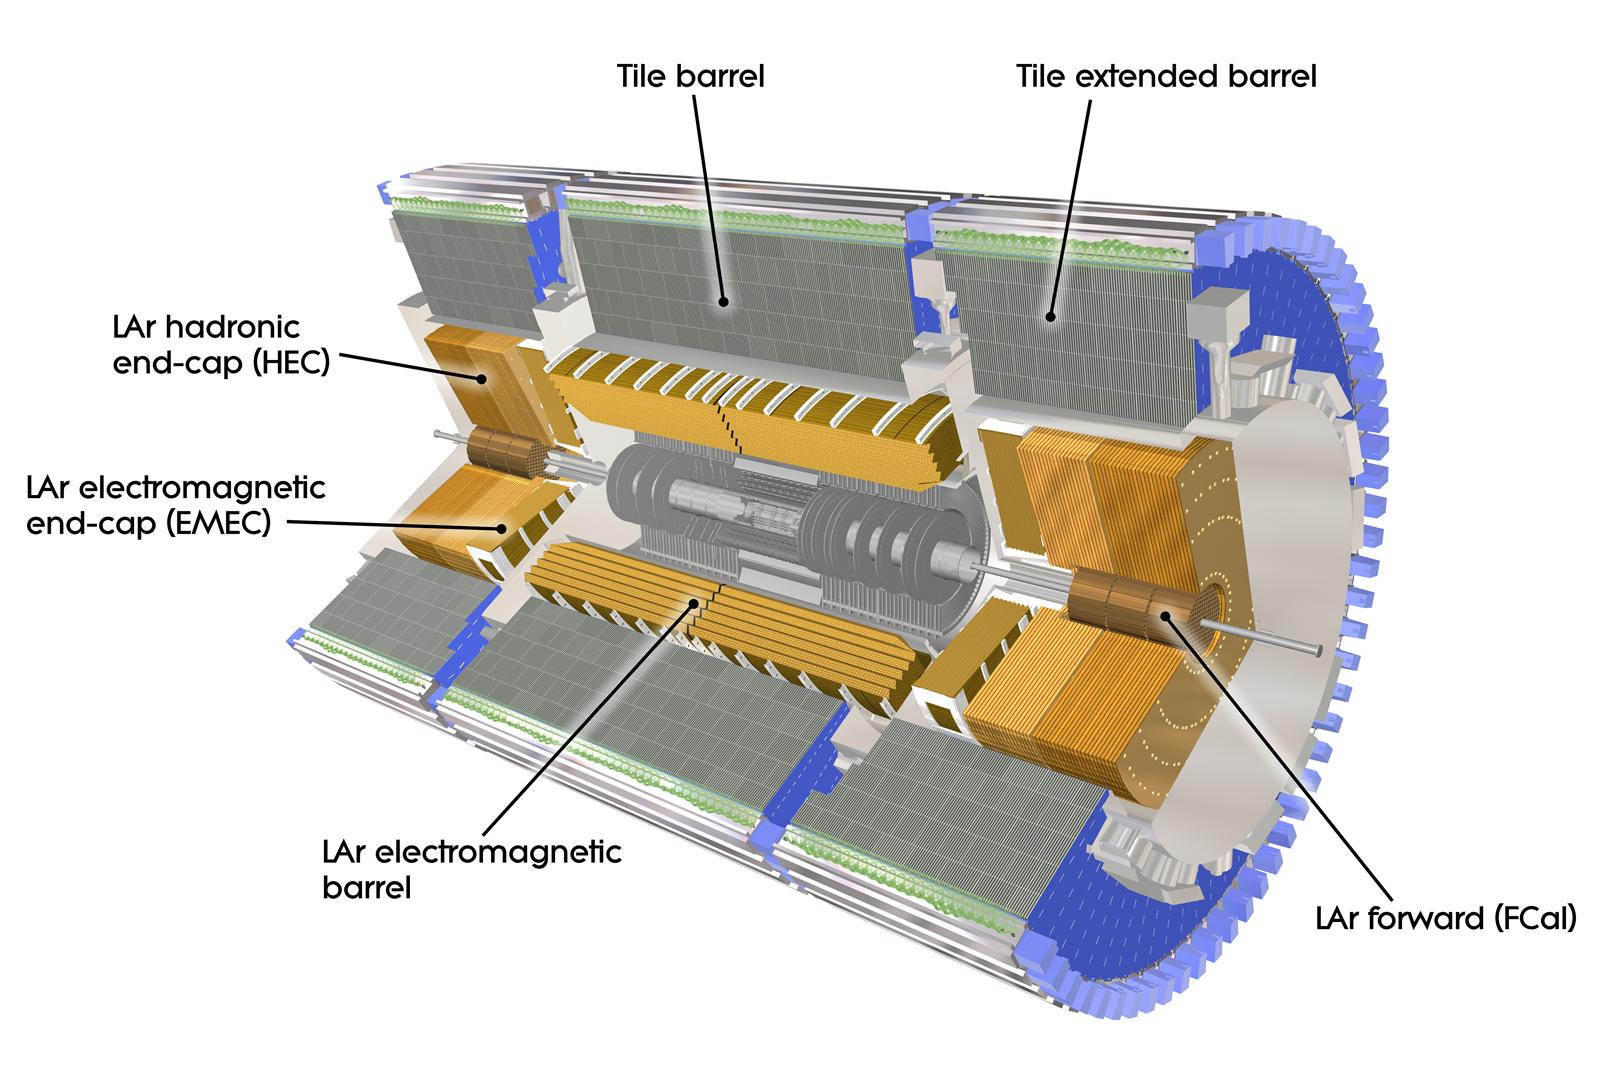
\includegraphics[scale=0.4]{0803015_01-A4-at-144-dpi.jpg}
        \caption{Cut-away view of the calorimeter system~\cite{Aad:2008zzm}.}
        \label{fig:ae_calorimeter}
    \end{center}
\end{figure}

%%%
%%%
%%%

\subsubsection{Electromagnetic calorimeter}
\label{subsubsec:ae_ecal}
The \textit{electromagnetic calorimeter} (ECAL) measures the energy of electrons and photons as they interact with matter.
The ECAL consists of accordion shaped cells of alternating layers of lead as absorber material and liquid argon (LAr) as active medium.
The accordion shaped provides the full coverage in the azimuthal angle $\phi$.
The LAr is chosen as an active medium because it is hard to radiate, it has stable response time and linear behaviour~\cite{Aad:2008zzm}.
The electrons or photons lose their energies by alternating bremsstrahlung and pair production when they interact with lead and result in the electromagnetic particle showers which ionise the LAr and the ionisation currents are collected by the copper electrodes.
The ECAL is divided into barrel (EMB) and end-cap (EMEC) components, which cover $|\eta| < 1.475$ and $1.375 < |\eta| < 3.2$\footnote{There are two EMECs and each of them consists of two wheels. The inner wheel covers $1.375 < |\eta| < 2.5$ and the outer wheel covers $2.5 < |\eta| < 3.2$.}, respectively.
The EMB is made up of three longitudinal layers with different granularity and sensitive in the region $|\eta| < 2.5$.
The first strip layer has the highest granularity where the size of cells corresponding to $\Delta \eta \times \Delta \phi = 0.0031 \times 0.1$ for $|\eta| < 1.8$ and coarser for larger $|\eta|$.
The smallest granularity allows to separate the showers coming from electrons, photons and neutral pions.
The second layer is the largest part of the EMB with the size of cells corresponding to $\Delta \eta \times \Delta \phi = 0.025 \times 0.0245$ so most of the energies are deposited in this layer.
The third layer has the granularity $\Delta \eta \times \Delta \phi = 0.05 \times 0.0245$.
The total thickness are 22~$X_{0}$\footnote{The $X_{0}$ stands for radiation lengths which is a characteristic of material. It is related to the energy loss of the particle when it interacts with the material electromagnetically.} and 24~$X_{0}$ for EMB and EMECs, respectively.
This special thickness is sufficient to prevent the punch-throughs of high energy showers into the muon spectrometer.
Figure~\ref{fig:ae_ecal} shows the cut-away view of the the accordion shaped EMB module with the dimensions for three layers.

\begin{figure}[htbp]
    \begin{center}
        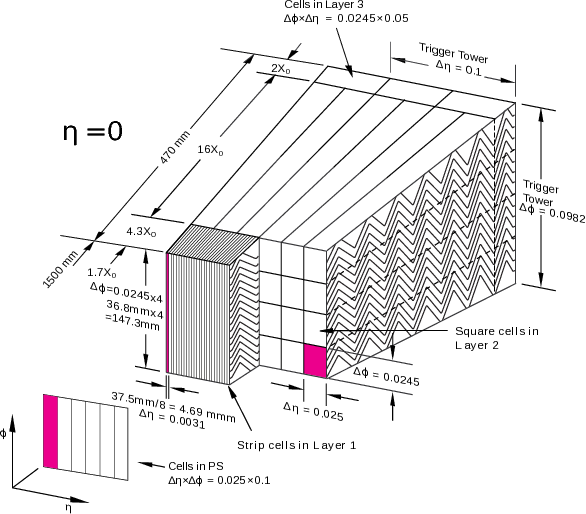
\includegraphics[scale=0.5]{LARG3-TDR-barrelM_samplings_presamp_new.png}
        \caption{Cut-away view of the accordion shaped EMB module with the dimensions for three layers~\cite{Strizenec:2014ida}.}
        \label{fig:ae_ecal}
    \end{center}
\end{figure}

%%%
%%%
%%%

\subsubsection{Hadronic calorimeter}
\label{subsubsec:ae_hcal}
The electromagnetic interacting particles produce narrow showers, however, the hadrons, which are heavier and penetrate medium further, produce more wide-spread hadronic showers.
The \textit{hadronic calorimeter} (HCAL) surrounds the ECAL and is made up by a barrel and two end-caps  (HEC).
The barrel covers $|\eta| < 1.7$ and it uses plastic scintillator tiles as active medium and steel as absorber material.
The hadronic showers stimulate the scintillator and emit light which is collected by \textit{photo multiplier tubes} (PMTs) and then read-out via wavelength shifting optical fibers. 
The HEC covers $1.5 < |\eta| < 3.2$ which overlap with the pseudorapidity coverage region of barrel.
The HEC is composed of two copper plate wheels as absorber material on each side and the LAr in between.
The designed thickness in the barrel region is 9.7~$\lambda$\footnote{The $\lambda$ represents the hadronic interaction lengths which is the mean free path of a strongly interacting particle between two inelastic scatterings.}.
Therefore, the punch-through to the muon spectrometer is suppressed.
The granularity of the HCAL is coarser than the ECAL but it is sufficient for measuring \met and jet reconstruction.

%%%
%%%
%%%

\subsubsection{Forward calorimeter}
\label{subsubsec:ae_fcal}
The \textit{forward calorimeter} (FCAL) uses the LAr as active medium and one copper and two tungsten layers as absorber materials.
The copper layer (FCAL1) is used to measure the electromagnetic interactions whereas the two tungsten layers (FCAL2 and FCAL3) is used to measure the hadronically interactions.
The FCAL provides the very forward region coverage $3.1 < |\eta| < 4.9$ can contribute the \met measurement.

%%%
%%%
%%%

\subsubsection{Energy resolution}
\label{subsubsed:ae_energy_resolution}
The energy resolution is the ability of the calorimeter to distinguish the two adjacent energies.
The number of ionized particles $N$ is proportion to the energy $E$ of the incoming particle.
%
%\begin{equation}
%   N \propto E
%   \label{eq:ae_number_of_ionized_particles}
%\end{equation}
%
Therefore, the higher energy of the incoming particle the more ionised particles produced in the shower.
Based on the Poisson statistics we know
%
\begin{equation}
    \frac{\sigma_{E}}{E} \propto \frac{\sigma_{N}}{N} = \frac{\sqrt{N}}{N} = \frac{1}{\sqrt{N}} \propto \frac{1}{\sqrt{E}}
    \label{eq:ae_energy_resolution}
\end{equation}
%
where $\sigma_{E}$ is the energy resolution at FWHM\footnote{The FWHM means full width at half maximum.} in a Gaussian distribution and $\sigma_{N} = \sqrt{N}$ is the Poisson standard deviation.
Taking the effects of calibration and electronics noise into account, the relative energy resolution becomes
%
\begin{equation}
    \frac{\sigma_{E}}{E} = \frac{a}{E} \oplus \frac{b}{\sqrt{E}} \oplus c
    \label{eq:ae_relative_energy_resolution}
\end{equation}
%
where $a, b, c$ are noise, sampling, and constant terms, respectively.
The relative energy resolutions for ECAL, HCAL, and FCAL are summarised in Table~\ref{tab:ae_relative_energy_resolution}.

\begin{table}[htbp]
    \begin{center}
        {\footnotesize
            \begin{tabular}{cc}
                \hline
                \hline
                Calorimeter                 & Required resolution\\
                \hline
                Electromagnetic calorimeter & $\sigma_{E}/E = 10\% / \sqrt{E\mathrm{ (GeV)}} \oplus 0.7\%$\\
                Hadronic calorimeter        & $\sigma_{E}/E = 50\% / \sqrt{E~\mathrm{(GeV)}} \oplus 3\%$\\
                Forward calorimeter         & $\sigma_{E}/E = 100\% / \sqrt{E~\mathrm{(GeV)}} \oplus 10\%$\\
                \hline
                \hline
            \end{tabular}
        }
    \end{center}
    \caption{Resolution requirements for the different calorimeters of the ATLAS detector~\cite{Aad:2008zzm}.}
    \label{tab:ae_relative_energy_resolution}
\end{table}%

%%%
%%%
%%%

\subsection{The muon spectrometer}
\label{subsec:ae_the_muon_spectrometer}
The outermost part of the ATLAS detector is the \textit{muon spectrometer}~\cite{Aad:2008zzm, Palestini:2003dm, Diehl:2009bw}.
Muons have the same properties as electrons but 200 times heavier than the electrons.
Because muons don't interact predominately by bremsstrahlung, most of the muons escape the inner detector and calorimeters without being stopped.
Only the muons with an energy less than 5~{\GeV} are stopped before the muon spectrometer.
Therefore, a detector concentrates on the measurement of high precision momentum and trajectory of muons is necessary.
%Therefore, muons are the only measurable particles that can penetrate the inner detector and the calorimeters.
%In order to determine the momentum with high precision and trajectory of muons, a detector that concentrates on the measurement of muons is necessary.

The muon spectrometer is designed to measure the transverse momentum ($p_{\mathrm{T}}$) of muons with $p_{\mathrm{T}} > 3$~{\GeV} with a resolution of 3\% for $p_{\mathrm{T}} < 250$~{\GeV} and increasing to 10\% at 1~{\TeV}.
It consists of large toroid magnets system and high precision tracking chambers allowing a precise measurement of the muon momentum over nearly the full solid angle.
The barrel toroid magnet system is composed of eight superconducting coils which are installed radial symmetrically around the beam pipe.
It covers the range $|\eta| < 1.4$ and bends the trajectories of muons with the bending power 1.5 to 5.5 Tm.
The magnetic field produced by the barrel toroid magnets provides an approximately 1~T field at the center of each coils, but is rather non-uniform, especially in the barrel-endcap transition region.
In the endcap toroid magnets system, the magnetic field is provided by eight superconducting coils, closed in an insulation vessel extending to about 10 m in diameter, located between the first and the second station of tracking chambers.
The endcap toroid magnets cover $1.6 < |\eta| < 2.4$ and provide a magnetic field in the range of 1 to 2 T with bending power 1 to 7.5 Tm.

The \textit{monitored drift tubes} (MDT) consists of cylindrical drift tubes, filled with a gas mixture of Ar and CO$_{2}$.
A tungsten-rhenium alloyed aluminium wire in the centre of each tube collects the electrons freed by ionisation of the gas volume by traversing muons.
The MDT covers a full range of $|\eta| < 2.7$, while the inner layer only covers $|\eta| < 2.0$.
The \textit{cathode strip chambers} (CSC) provides a coverage range $2.0 < |\eta| < 2.7$, where MDTs would have occupancy problems.
The CSC is made up by two discs and filled with Ar and CO$_{2}$ gas mixture.
Both MDT and CSC are slow for trigger but they provide high precision tracking in the spectrometer bending plane and end-cap inner layer, respectively.
The \textit{resistive plate chambers} (RPC) and \textit{thin gap chambers} (TGC) are used for triggering in barrel and end-cap, they have sufficient intrinsic time resolution of 1.5 ns and 4 ns, respectively.
A sketch of the muon spectrometer and its four components are depicted in Figure~\ref{fig:ae_muon_spectrometer} and Table~\ref{tab:ae_muon_spectrometer_components} gives a summary of the muon spectrometer components.

\begin{figure}[htbp]
    \begin{center}
        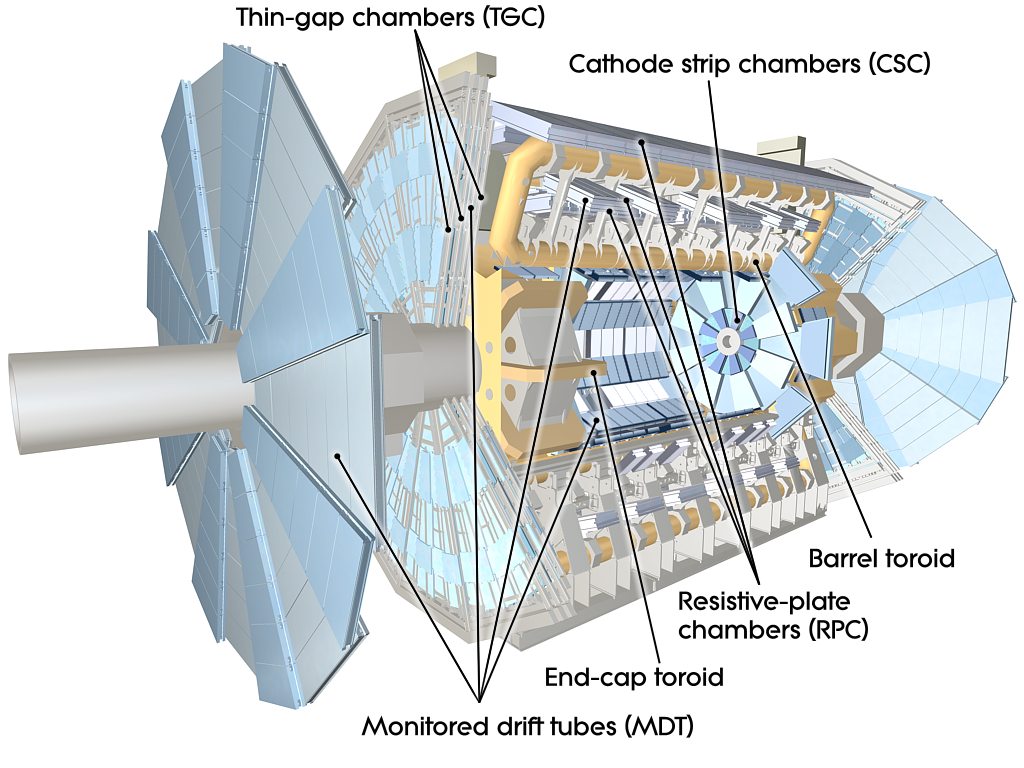
\includegraphics[scale=0.3]{MuonSystem_d3.png}
        \caption{Sketch of the muon system of the ATLAS detector~\cite{Aad:2008zzm}.}
        \label{fig:ae_muon_spectrometer}
    \end{center}
\end{figure}

\begin{table}[htbp]
    \begin{center}
        {\footnotesize
            \begin{tabular}{ccccc}
                \hline
                \hline
                Type & Purpose  & Location         & $\eta$ coverage    & Channel\\
                \hline
                MDT  & Tracking & barrel + end-cap & $0.0 < \eta < 2.7$ & 354k\\
                CSC  & Tracking & end-cap layer 1  & $2.0 < \eta < 2.7$ & 30.7k\\
                RPC  & Trigger  & barrel           & $0.0 < \eta < 1.0$ & 373k\\
                TGC  & Trigger  & end-cap          & $1.0 < \eta < 2.4$ & 318k\\
                \hline
                \hline
            \end{tabular}
        }
    \end{center}
    \caption{A summary of the muon spectrometer components.}
    \label{tab:ae_muon_spectrometer_components}
\end{table}%

%%%
%%%
%%%

\subsection{The trigger system and data acquisition}
\label{subsec:ae_trigger}
The LHC $pp$ collision rate is 40~MHz corresponding to 50~TB/s data\footnote{Assuming the typical event size is 1.3~MB.} generated by the ATLAS detector~\cite{Kordas:2007zz}.
However, the limited rate for writing the events into disk is about 1~kHz\footnote{The data storage rate is 200~Hz in Run-1 but it is increased to about 1~kHz in Run-2.}.
The majority of the products of the $pp$ collision are low \pt QCD processes which are not the interesting events for the analysis.  
Hence, the three-level ATLAS trigger and data acquisition (DAQ) system is designed to pick the interesting events and reduce the data size.
Figure~\ref{fig:ae_tdaq} shows the functional view of the ATLAS trigger/DAQ system and the brief descriptions are given in the following paragraph.

\begin{figure}[htbp]
    \begin{center}
%       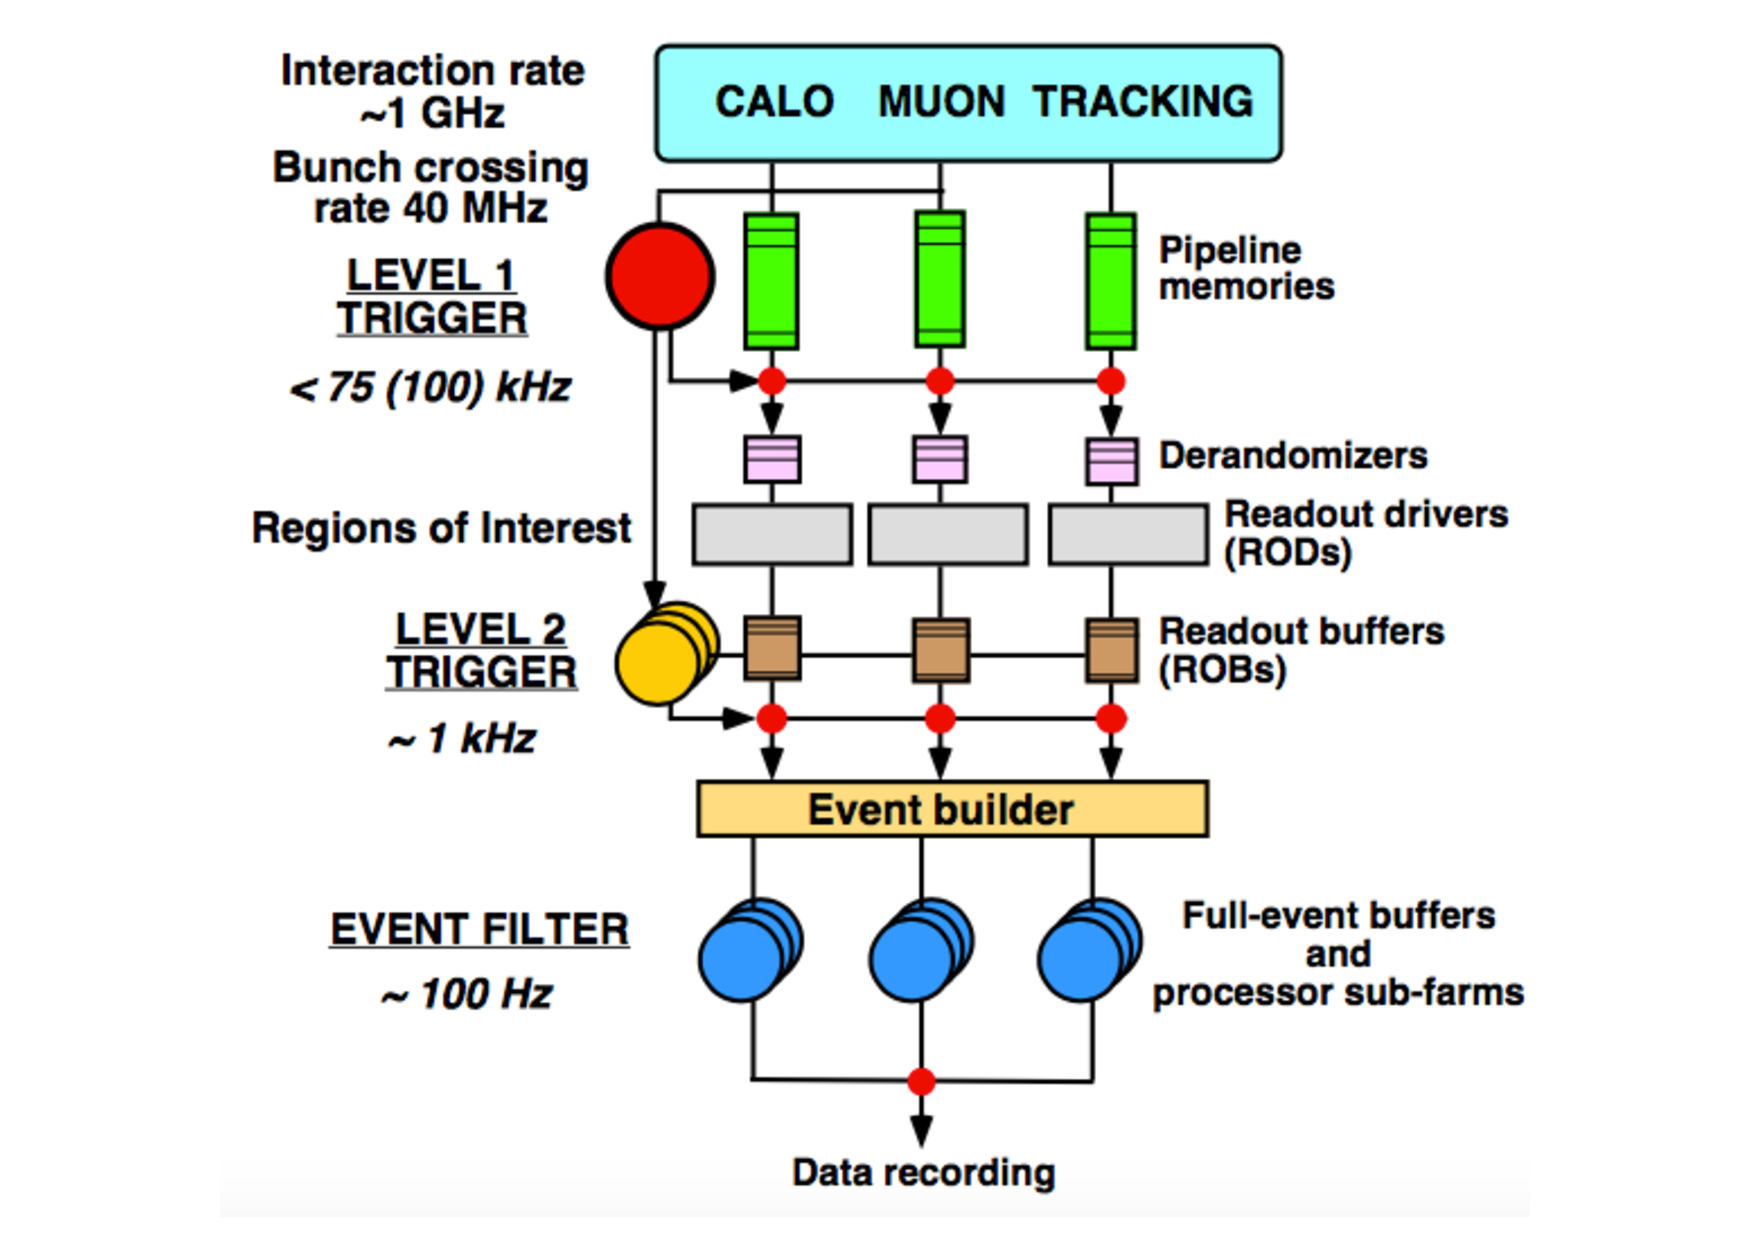
\includegraphics[scale=0.4]{ATLAS_TDAQ.pdf}
%       \caption{The functional view of the ATLAS trigger/DAQ system.
%       The figure is taken from~\cite{ATLAS:1999uwa}.}
        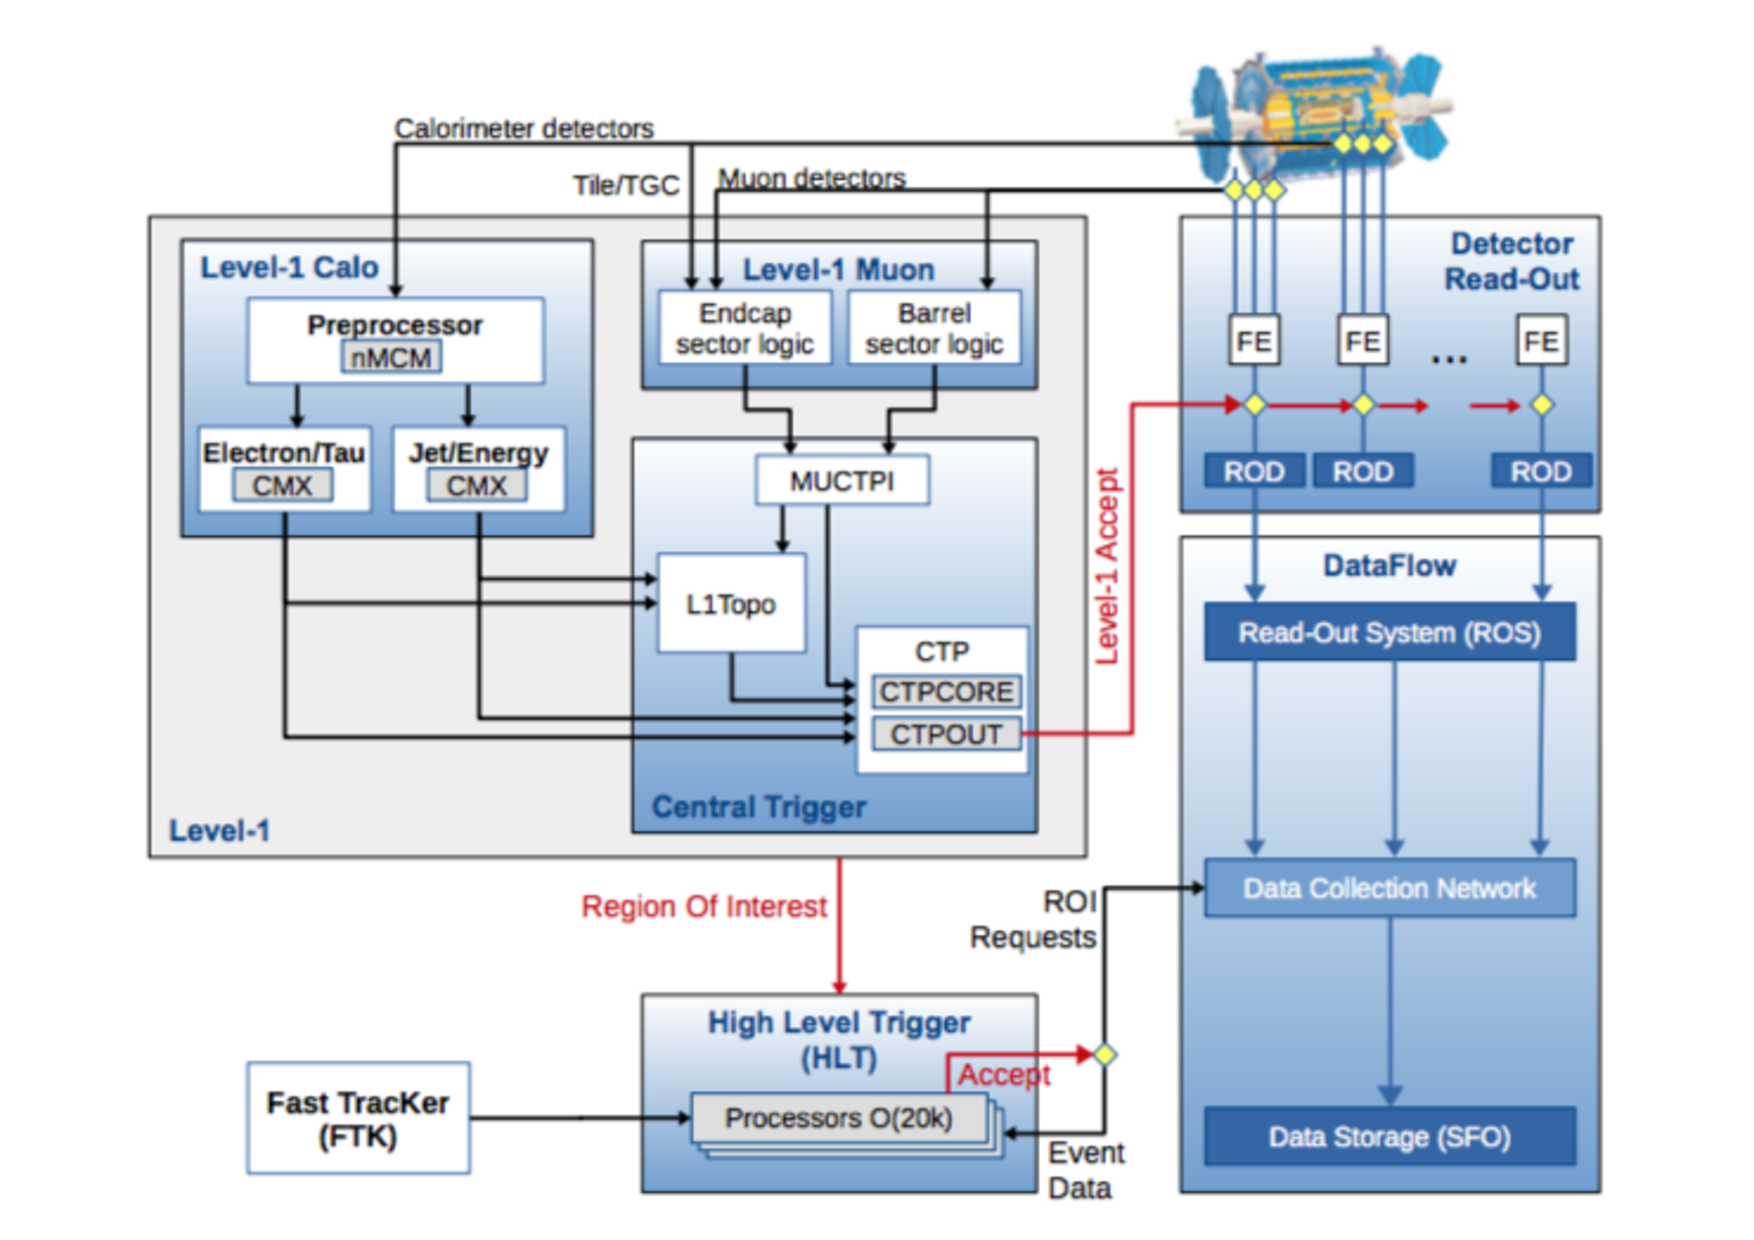
\includegraphics[scale=0.39]{ATLAS_TDAQ_Run2.pdf}
        \caption{The schematic view of the ATLAS trigger/DAQ system in Run-2.
        The figure is taken from~\cite{Martinez:2016udm}.}
        \label{fig:ae_tdaq}
    \end{center}
\end{figure}

%%%
%%%
%%%

\subsubsection{The level-1 trigger}
\label{subsubsec:ae_LVL1}
The initial selection is made by the hardware-based \textit{level-1} (LVL1) trigger based on reduced-granularity information from calorimeters and the muon spectrometer.
The latency\footnote{The latency is the time interval from the $pp$ collision until trigger decision is available to the front-end electronics.} of the level-1 trigger is required to be less than 2.5~$\mu s$\footnote{The target latency for the level-1 trigger is 2.0~$\mu s$.}.
The high \pt muons are identified using only RPC and TGC.
The high \pt $e/\gamma$, jets, hadronically decaying $\tau$-leptons, large \met and total \et objects are selected by calorimeter trigger using a number of sets of \pt thresholds\footnote{Typically, there are 6 to 8 sets of thresholds per object type.} and the energy isolation cuts can be applied. 
The selected events are read out from the front-end electronics into \textit{readout drivers} (RODs) and written into \textit{readout buffers} (ROBs).
The information such as the \pt, $\eta$, and $\phi$ of the candidate objects and \met and total \et are saved into \textit{region-of-interest} (ROI) and send to the high level trigger.
The level-1 trigger reduces the event rate from the high LHC bunch crossing rate to 100~kHz.

%%%
%%%
%%%

\subsubsection{The high level trigger}
\label{subsubsec:ae_HLT}
The \textit{level-2} trigger and \textit{event filter} (EF) computer clusters used in Run-1 are merged into a single event professing \textit{high level trigger} (HLT) farm in Run-2.
This combination reduces the complexity, allows resource sharing between algorithms, and results in a more flexible HLT.
The HLT is completely software based trigger system and it uses the ROI information from the level-1 trigger and the tracking information from the inner detector.
The full-event track reconstruction information is performed by the \textit{fast tracker} (FTK) system after each level-1 trigger and provided to the HLT.	 
The trigger reconstruction algorithms for HLT were re-optimised to minimise the differences between the HLT and the offline analysis selections.
The output rate of the HLT is approximately 1~kHz within a processing time about 200~$\mu s$.
